\subsection{Scrum of scrums}\label{sub:scrum-of-scrums}
Scrum of Scrums is a framework for scaling scrum across an organization. 
The ECDAR-SW5 organization uses Scrum of Scrums, as it allows each scrum team freedom to operate independently while providing a structure for communication \cite{spanner_scrum_nodate}. 

%In scrum of scrums we do not have daily scrums because the daily scrums is held in the smaller groups.
The daily scrum is a daily event, and because of that it would be impossible to get everyone together in the scrum of scrums every day for a daily scrum meeting.
Based on that we do not have daily scrums in the scrum of scrums.
%Working in scrum of scrums allows us as an organization to only hold daily scrum in each individual group, rather than across the entire organization.
%This simplifies the entire work process, ensuring focus. 
The key events in scrum of scrums are the sprint planning, sprint review, and sprint retrospective, and these events are handled by representatives of each group, which ensures that all groups have some insight into the overall process.
See \autoref{fig:scrum-of-scrums-events} for a more detailed look of the different events between scrum and scrum of scrums.

The multi-project is separated into two parts. 
There are five project groups working with the Reveaal engine, and one group working with GUI.
Each group has chosen a member to attend the scrum of scrums meetings as a representative of the group.
The reasoning for this was the number of members attending the meetings would get to big if every group member attended. 
The idea behind this was to keep the meetings as short as possible, and because of this, each group should hold a meeting internally after the sprint planning and before the review and retrospective. This ensures the representative is ready for the main scrum of scrums meeting. This process is also described in the figure below \ref{fig:scrum-of-scrums-events}.

%sending their committee to the main meeting for the scrum of scrums. 
%Based on that the groups choose a committee to attend the scrum meetings.

\begin{figure}[H]
    \centering
    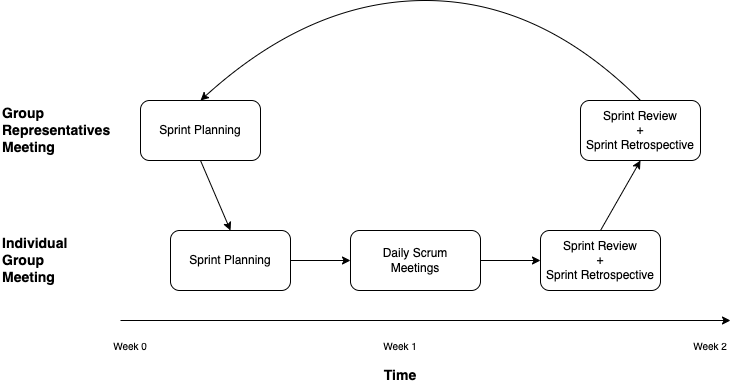
\includegraphics[width=\textwidth]{common/figures/Scrum_of_scrums_schedule.png}
    \caption{A figure depicting the events in a scrum sprint, divided between the big scrum of scrums group and the smaller scrum groups.}
    \label{fig:scrum-of-scrums-events}
\end{figure}


As mentioned, the multi-project focuses on both the GUI and Reveeal engine.
Because of this dual focus, we have two product owners: one product owner for the Reveaal teams and one for the GUI team.
The project's different product owners will help upholding the product backlog and update it if any changes appears. 
These changes are discussed during the scrum of scrums meetings, where the product owners can also be present.

The length of a sprint is measured against the length of the smaller scrum group's sprints.
Because of this, the average sprint length is two weeks.
Based on the length of the sprint, the scrum of scrums group has two meetings every two weeks. 
One meeting is for planning the upcoming sprint, and one is for sprint reviewing and retrospective at the end of a sprint.
These meetings, if possible, are held on the first Monday of a sprint, and the last Friday of a sprint, respectively.

% One for planing the upcoming sprint the first monday of the sprint, if possible and one meeting on last friday of the sprint, if possible.
% The last meeting's topics are always sprint reviewing and sprint retrospecting. 

\subsubsection{The Mutual Definition of Done}\label{common:collaboration:DoD}
To better facilitate multiple Scrum teams working on the same codebase, a Definition of Done (DoD) is necessary. The objective of defining a DoD is to have a shared agreement of when a feature is done, this shared definition was described in the first Scrum of Scrums meeting.

The definition we settled on was that every pull request to the GUI- and Reveaal-repositories' main-branches should be reviewed internally in the team as a draft, before it is sent out for an external review.
The external review consists of four different checks:
\begin{itemize}
    \item Ensure the new functionality described is implemented and works.
    \item Run a benchmark on the main- as well as the new functionalities branch.
    \item Check if the new code is properly documented. The I/O and panic criteria should be documented as well as what it does if functions are public.
    \item All tests should pass and if there is a new functionality it should be tested. It is up to the reviewers to judge if the tests are good enough.
\end{itemize}
Secondly the new functionality should be approved by two external reviewers.
%The external review consists of two people from other teams that follow a defined review guide which includes checks on functionality, performance, documentation, and tests.
If none of these areas are found lacking, and both reviewers approve of the changes, it is considered done.

It is worth noting that we have not made a formal definition for anything other than the code. However a review process for the collaborative part of the report exists. The review process is threefold, each Scrum team separately reviews the report. Thereafter each teams is assigned an area of responsibility, which is corrected and proof read. Lastly the original person/team who commented on the now corrected part, either accepts the change, or contacts the person who made it. After this process, the collaborative writing is considered done.
Any other DoD will be at the individual team's discretion to create.


% The mutual definition of DoD between the Scrum groups is:
% \begin{itemize}
%     \item Each increments should be reviewed by two students from the Scrum of Scrums.
%     \item Increments shall reviews internally in the group before making a pull request on Github.
%     \item If a increment is not reviewed in less than a day, the groups have failed to uphold their commitment to review other pull requests. 
%     \item Write code documentation that fits the written code. Such that having i/o variables defined, panic criteria and what the function descriptions.
%     \item It is up to the reviewers of the pull requests to say if the code is tested enough. 
% \end{itemize}

